%!TEX root = ../paper.tex

% Hardly any difference between estimators
One of the most striking observations from \cref{s:results} is that the difference in performance between the two estimators is minimal. 
	
	% Study differences further mbe vs sambe plot
	Plotting the densities as estimated by \sambe as a function of those estimated by \mbe shows no interesting differences between the two estimators for dataset \ferdosiOne through \baakmanFive. 
		% Multi Sphere Sets
		However for dataset \ferdosiTwo through \baakmanThree these plots reveal some differences between estimators. As can be seen in \cref{fig:discussion:performance:two:mbevssambe}, using shape-adaptive kernels results in estimated densities that are generally higher than those estimated with a fixed-shape kernel for dataset \ferdosiTwo and \baakmanTwo. Reviewing the raw data shows that \sambe underestimates densities less than \mbe on points near the mean of `Trivariate Gaussian 1'. The kernels in this neighborhood are all slightly anisotropic, and have allowed the shape-adaptive estimator to use more data points, to better approximate the local densities. Thus showing that estimating the density with shape-adaptive kernels can be advantageous.
		%
		\begin{figure}
			\centering
			\begin{subfigure}{0.3\textwidth}
				\centering
				\includegraphics[keepaspectratio=true, width=\textwidth, height=0.23\textheight]{discussion/img/ferdosi_2_60000_mbe_sambe.png}
				\caption{Dataset \ferdosiTwo}
				\label{fig:discussion:performance:mbevssambe:ferdosi2}
			\end{subfigure}
			\begin{subfigure}{0.3\textwidth}
				\centering
				\includegraphics[keepaspectratio=true, width=\textwidth, height=0.23\textheight]{discussion/img/baakman_2_60000_mbe_sambe.png}
				\caption{Dataset \baakmanTwo}
				\label{fig:discussion:performance:mbevssambe:baakman2}
			\end{subfigure}	
			\caption{Plots of the densities estimated by \sambe as a function of those estimated by \mbe for dataset %
				\subref{fig:discussion:performance:mbevssambe:ferdosi2} % 
				\ferdosiTwo and %
				\subref{fig:discussion:performance:mbevssambe:baakman2} %
				\baakmanTwo.
			}
			\label{fig:discussion:performance:two:mbevssambe}
		\end{figure}
		
		% Ferdosi 3 / Baakman 3
		\Cref{fig:discussion:performance:four:mbevssambe} shows the opposite effect; the densities estimated by \sambe for dataset \ferdosiThree and \baakmanThree are generally lower than those estimated by \mbe. Reviewing the raw data shows that the points with the greatest differences between the two estimators lie near the mean of the `Trivariate Gaussian 3' in both dataset \ferdosiThree and \baakmanThree. The number of points used in the density estimate by \sambe is consistently lower and than those used by the fixed-shape estimator. Given the relatively high anisotropy of the kernels in that area we expect that this is due to the kernels reflecting fine local structures, that do not reflect the more global neighborhood. 
		%	
		\begin{figure}
			\centering
			\begin{subfigure}{0.3\textwidth}
				\centering
				\includegraphics[keepaspectratio=true, width=\textwidth, height=0.23\textheight]{discussion/img/ferdosi_3_120000_mbe_sambe.png}
				\caption{Dataset \ferdosiThree}
				\label{fig:discussion:performance:mbevssambe:ferdosi3}
			\end{subfigure}
			\begin{subfigure}{0.3\textwidth}
				\centering
				\includegraphics[keepaspectratio=true, width=\textwidth, height=0.23\textheight]{discussion/img/baakman_3_120000_mbe_sambe.png}
				\caption{Dataset \baakmanThree}
				\label{fig:discussion:performance:mbevssambe:baakman3}
			\end{subfigure}	
			\caption{Plots of the density estimated by \sambe as a function of those estimated by \mbe for dataset %
				\subref{fig:discussion:performance:mbevssambe:ferdosi3} % 
				\ferdosiThree and %
				\subref{fig:discussion:performance:mbevssambe:baakman3} %
				\baakmanThree.
			}
			\label{fig:discussion:performance:four:mbevssambe}
		\end{figure}

	% Where are the differences largest -> plots
	% Single Sphere
		\begin{figure}
			\centering
			\begin{subfigure}{0.23\textwidth}
				\centering
				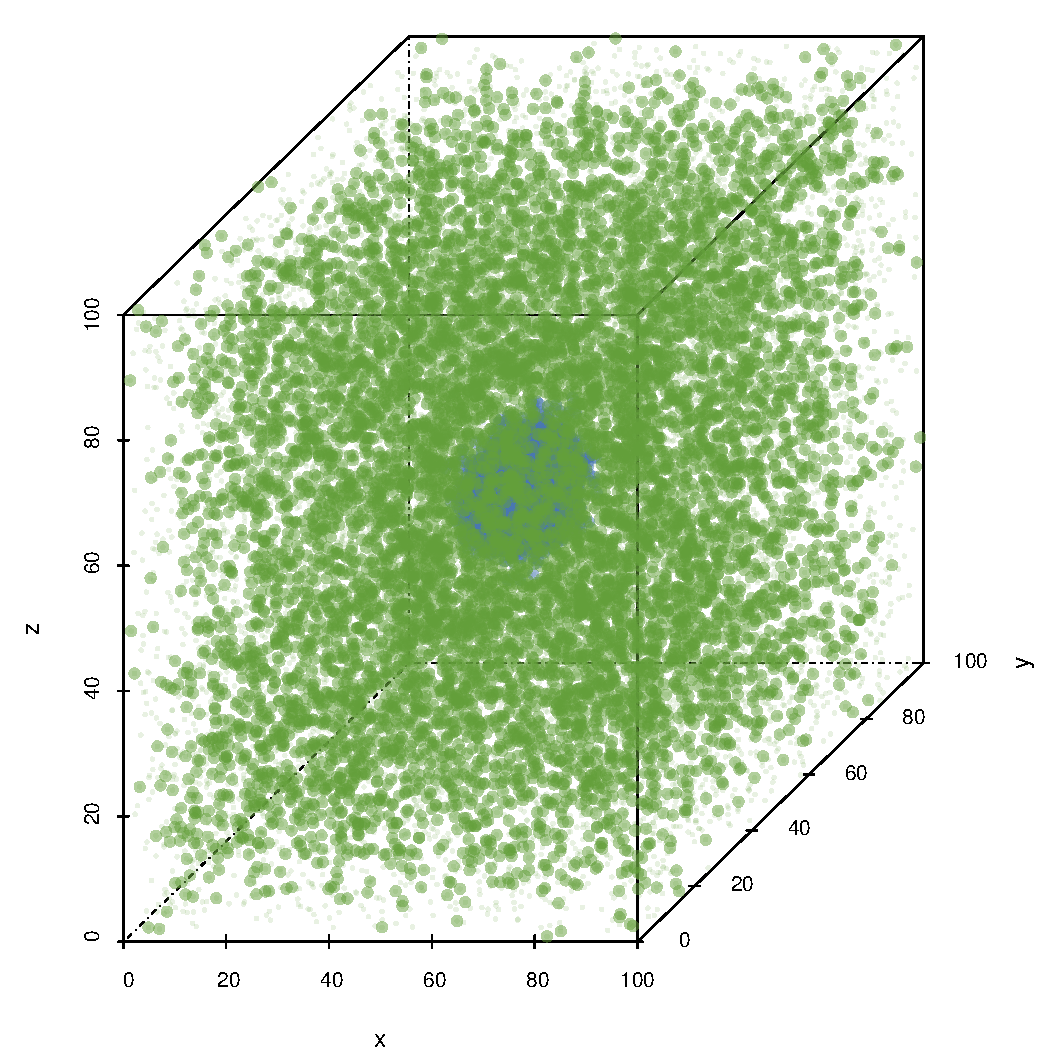
\includegraphics[keepaspectratio=true, width=\textwidth, height=0.23\textheight]{discussion/img/ferdosi_1_abs_error_mbeSmallerThansambe}
				\caption{Dataset \ferdosiOne}
				\label{fig:discussion:performance:mbeLowerError:ferdosi1}
			\end{subfigure}
			\begin{subfigure}{0.23\textwidth}
				\centering
				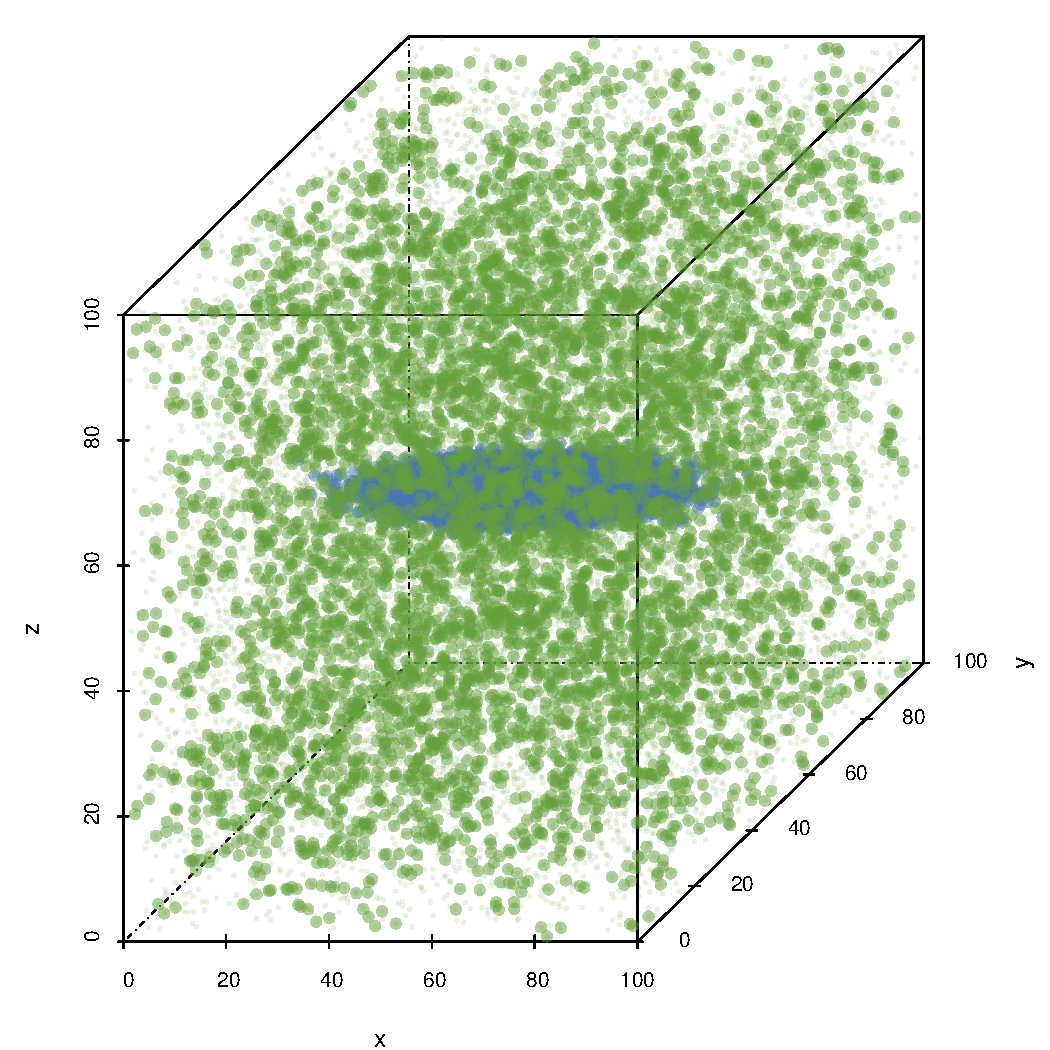
\includegraphics[keepaspectratio=true, width=\textwidth, height=0.23\textheight]{discussion/img/baakman_1_abs_error_mbeSmallerThansambe}
				\caption{Dataset \baakmanOne}
				\label{fig:discussion:performance:mbeLowerError:baakman1}
			\end{subfigure}	
			\begin{subfigure}{0.23\textwidth}
				\centering
				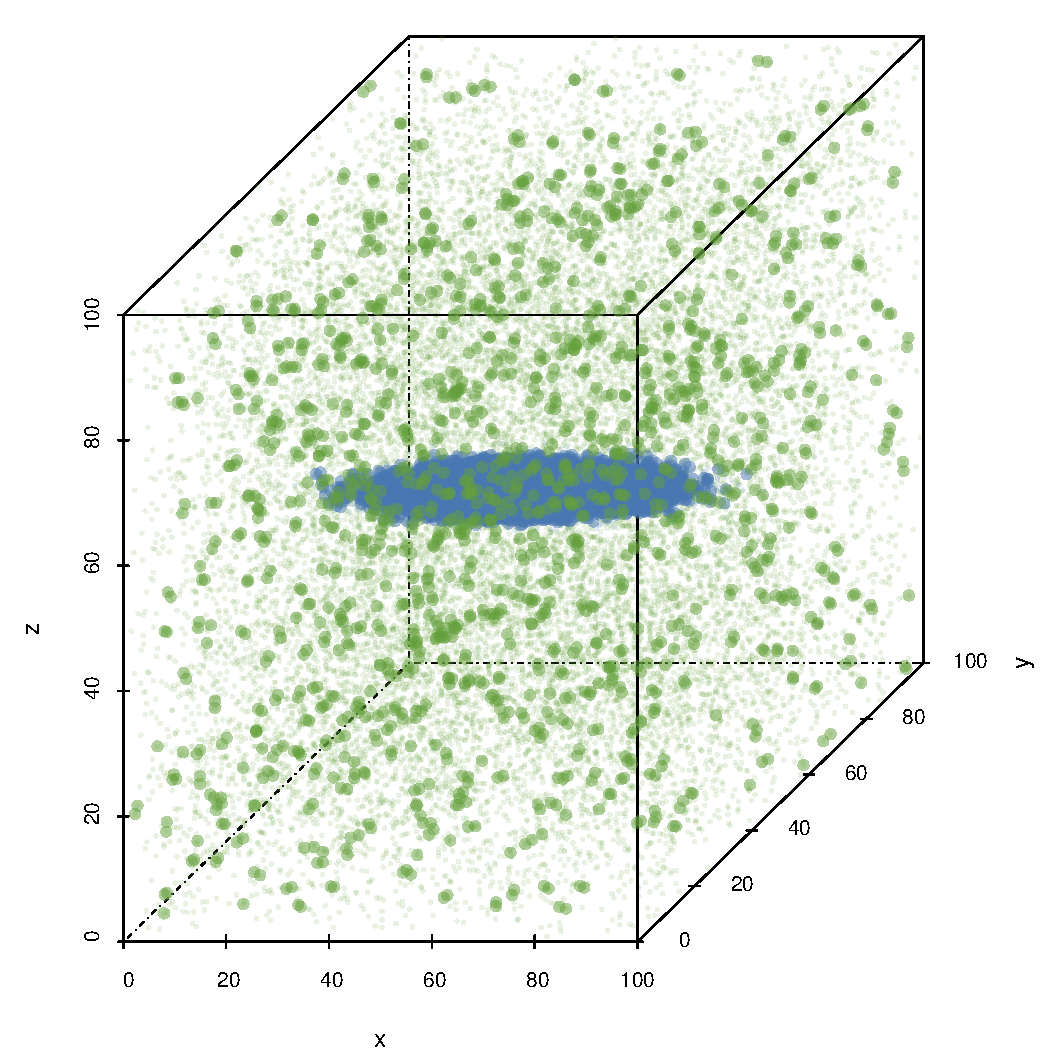
\includegraphics[keepaspectratio=true, width=\textwidth, height=0.23\textheight]{discussion/img/baakman_4_abs_error_mbeSmallerThansambe}
				\caption{Dataset \baakmanFour}
				\label{fig:discussion:performance:mbeLowerError:baakman4}
			\end{subfigure}		
			\begin{subfigure}{0.23\textwidth}
				\centering
				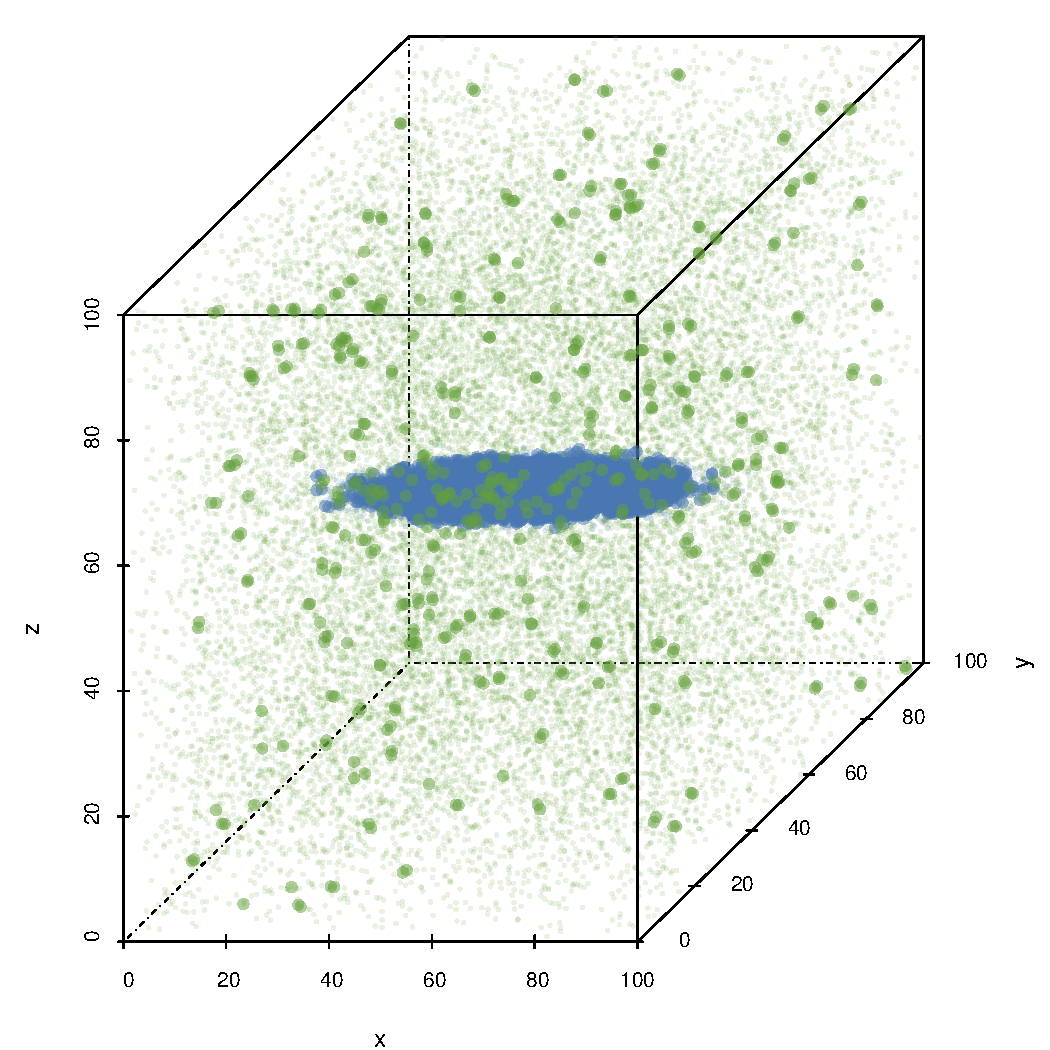
\includegraphics[keepaspectratio=true, width=\textwidth, height=0.23\textheight]{discussion/img/baakman_5_abs_error_mbeSmallerThansambe}
				\caption{Dataset \baakmanFive}
				\label{fig:discussion:performance:mbeLowerError:baakman5}
			\end{subfigure}			
			\caption{Low opacity scatter plot of dataset %
				\subref{fig:discussion:performance:mbeLowerError:ferdosi1} \ferdosiOne, %
				\subref{fig:discussion:performance:mbeLowerError:baakman1} \baakmanOne, %
				\subref{fig:discussion:performance:mbeLowerError:baakman4} \baakmanFour, and%
				\subref{fig:discussion:performance:mbeLowerError:baakman5} \baakmanFive, %
				with an overlay of larger colored points where the absolute error of \sambe is larger than the absolute error of \mbe.}
			\label{fig:discussion:performance:singleSphere:mbeLowerError}
		\end{figure}
		%	
		The plots in \cref{fig:discussion:performance:singleSphere:mbeLowerError} emphasize the points in dataset \ferdosiOne through \baakmanOne where the absolute error of \mbe is smaller than that of \sambe. These plots show that the shape-adaptive kernels outperform symmetric kernels near the borders of the datasets.
			% Why the boundary effect
			We expect that the boundary effect is due to the strong anisotropy of the local neighborhood of the points near the boundaries. Consequently the domain of the shape-adaptive kernels extends less outside of the boundaries dataset than the domains of the symmetric kernels. This results in less underestimation of densities near the boundary of the dataset, if shape-adaptive kernels are used.
			% Why is it stonger of the Gaussian is more anisotropic
			Furthermore the strength of the boundary effect seems to increase as the Gaussian component of the dataset is more anisotropic. However the seemingly better performance of \sambe is due to an increase in the number of points where the density estimated by \sambe equals the density estimated by \mbe. In dataset \ferdosiOne the density estimates of the two estimators differ on all points, in dataset \baakmanOne the estimators agree on the density of \percentage{1.327294605254362e+01} of the points, this increases to \percentage{3.535329901731399e+01} in dataset \baakmanFive.
			%SAMBE == MBE
			%Ferdosi 1 (0.000000000000000e+00 percent)
			%Baakman 1 (1.327294605254362e+01 percent)
			%Baakman 4 (2.989838892974129e+01 percent)
			%Baakman 5 (3.535329901731399e+01 percent)
			As the Gaussian component becomes more anisotropic the number of points whose local neighborhood consists only of uniform noise increases. On average the covariance matrix of neighborhoods that contain primarily points sampled from the noise component should be scalar. Consequently as the anisotropy of the Gaussian component increases more shape-adaptive kernels take on a shape that is near-symmetric. This results in points were both estimators give the same approximated density. 
	
	% Multi Sphere
		\begin{figure}
			\centering
			\begin{subfigure}{0.23\textwidth}
				\centering
				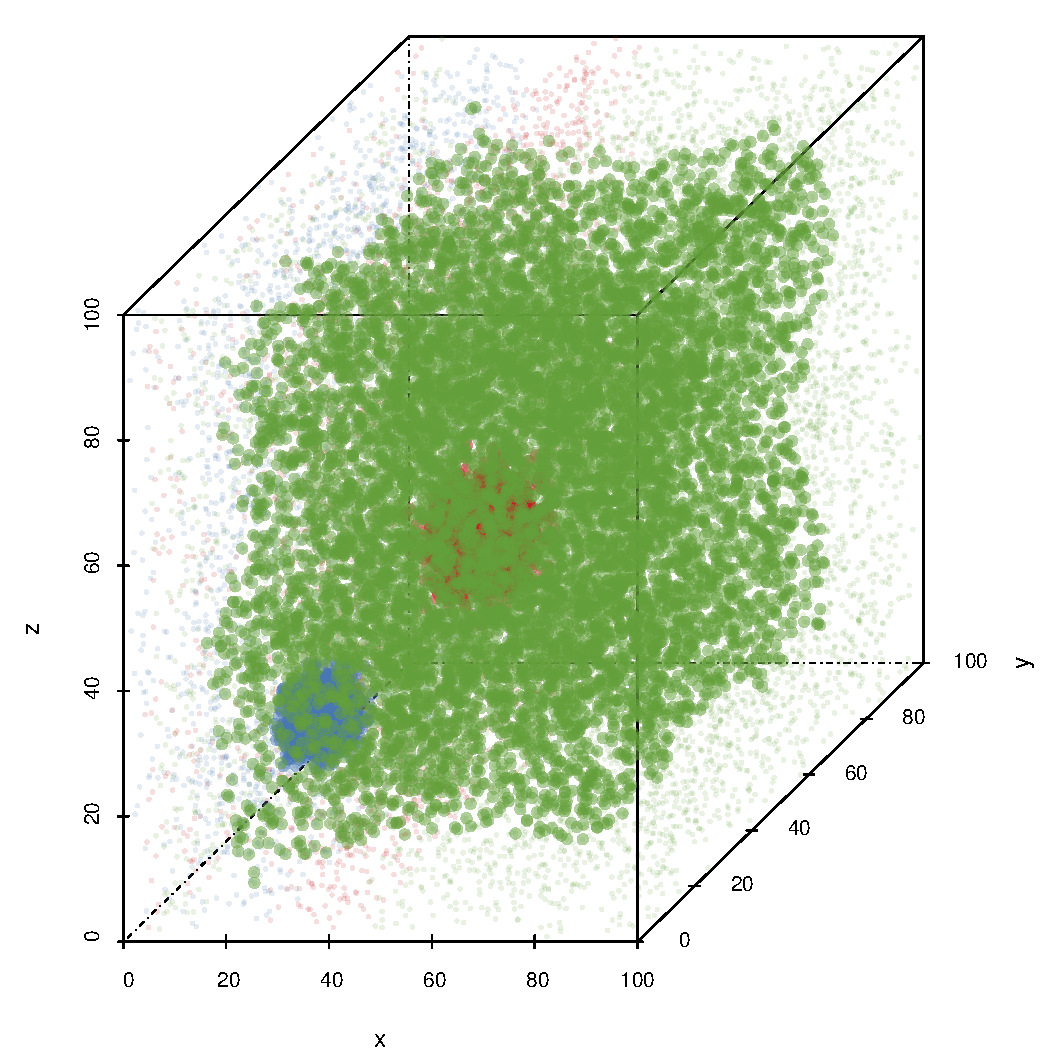
\includegraphics[keepaspectratio=true, width=\textwidth, height=0.23\textheight]{discussion/img/ferdosi_2_abs_error_mbeSmallerThansambe}
				\caption{Dataset \ferdosiTwo}
				\label{fig:discussion:performance:mbeLowerError:ferdosi2}
			\end{subfigure}
			\begin{subfigure}{0.23\textwidth}
				\centering
				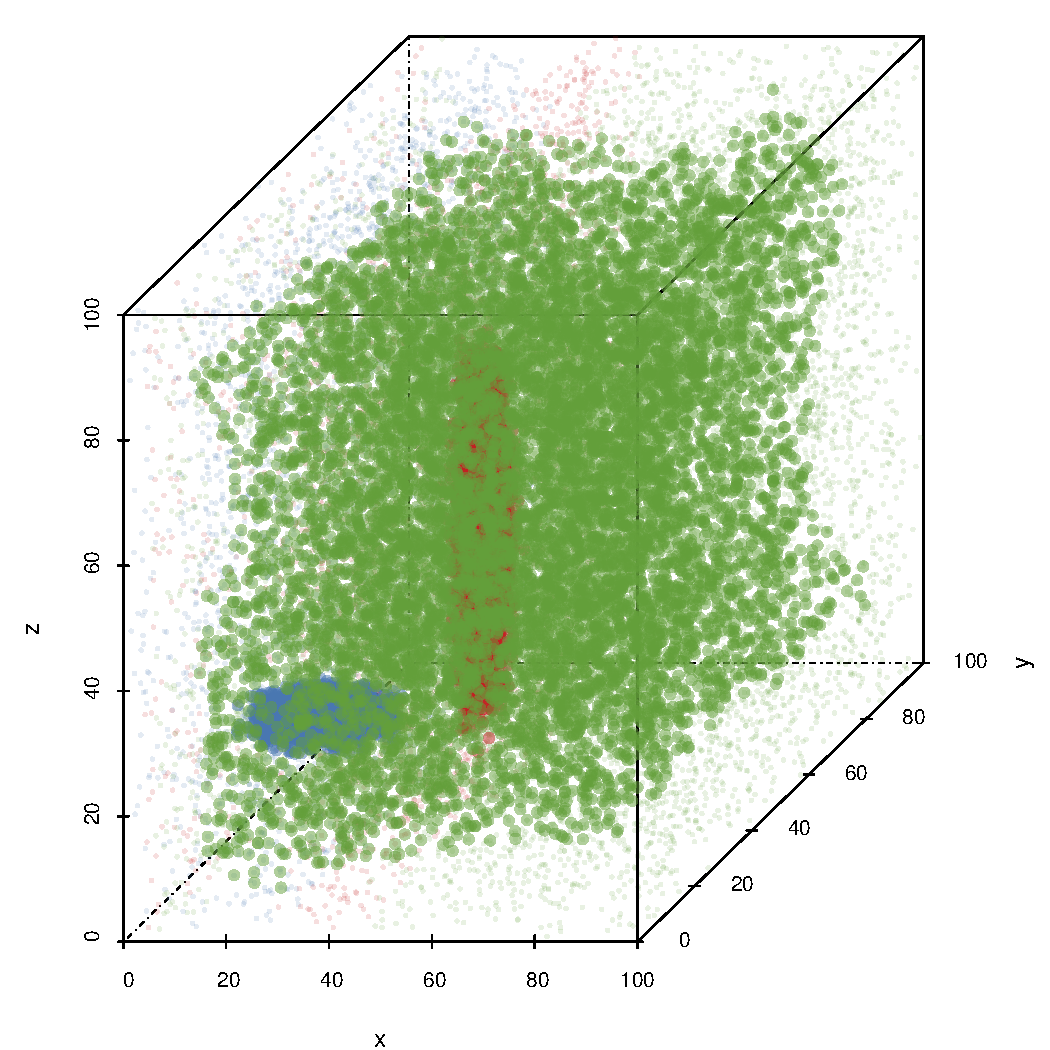
\includegraphics[keepaspectratio=true, width=\textwidth, height=0.23\textheight]{discussion/img/baakman_2_abs_error_mbeSmallerThansambe}
				\caption{Dataset \baakmanTwo}
				\label{fig:discussion:performance:mbeLowerError:baakman2}
			\end{subfigure}	
			\begin{subfigure}{0.23\textwidth}
				\centering
				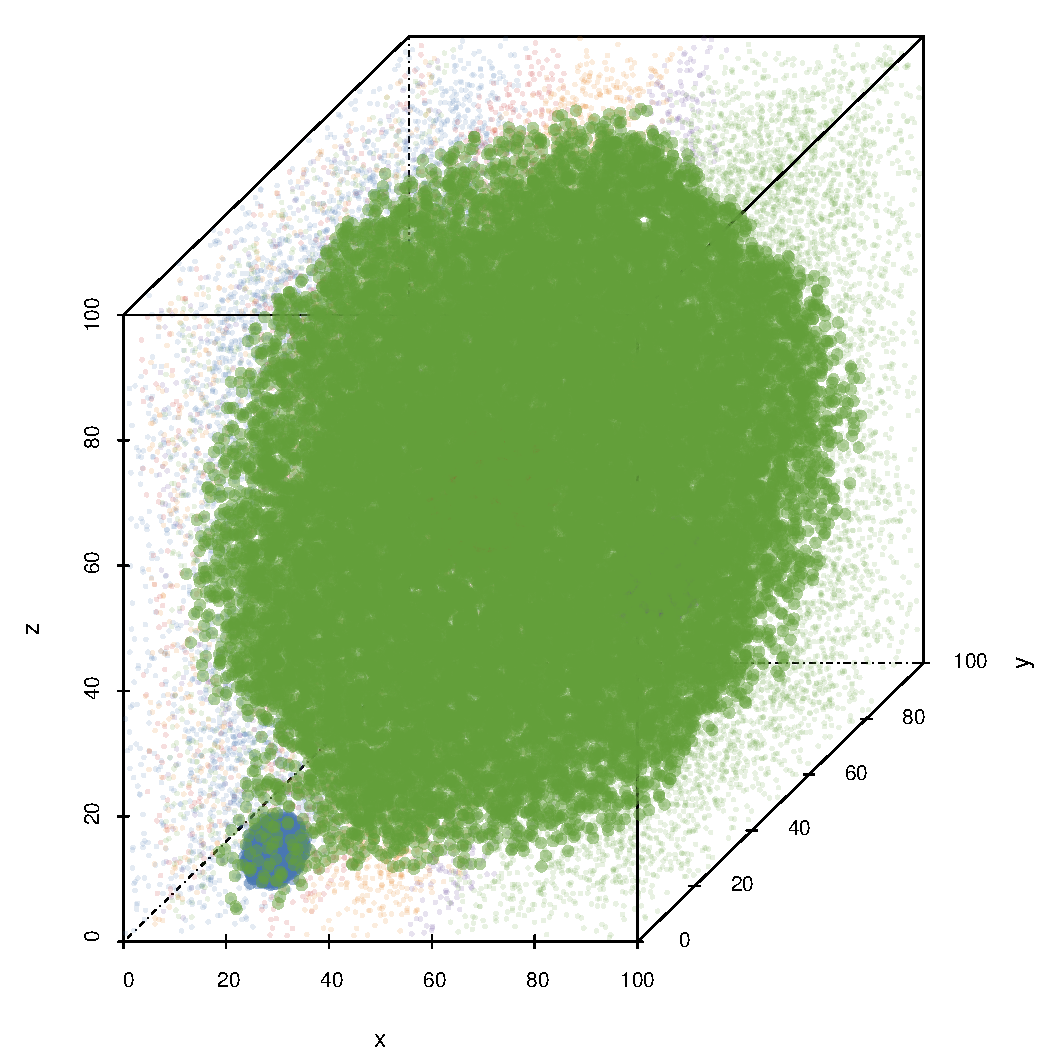
\includegraphics[keepaspectratio=true, width=\textwidth, height=0.23\textheight]{discussion/img/ferdosi_3_abs_error_mbeSmallerThansambe}
				\caption{Dataset \ferdosiThree}
				\label{fig:discussion:performance:mbeLowerError:ferdosi3}
			\end{subfigure}
			\begin{subfigure}{0.23\textwidth}
				\centering
				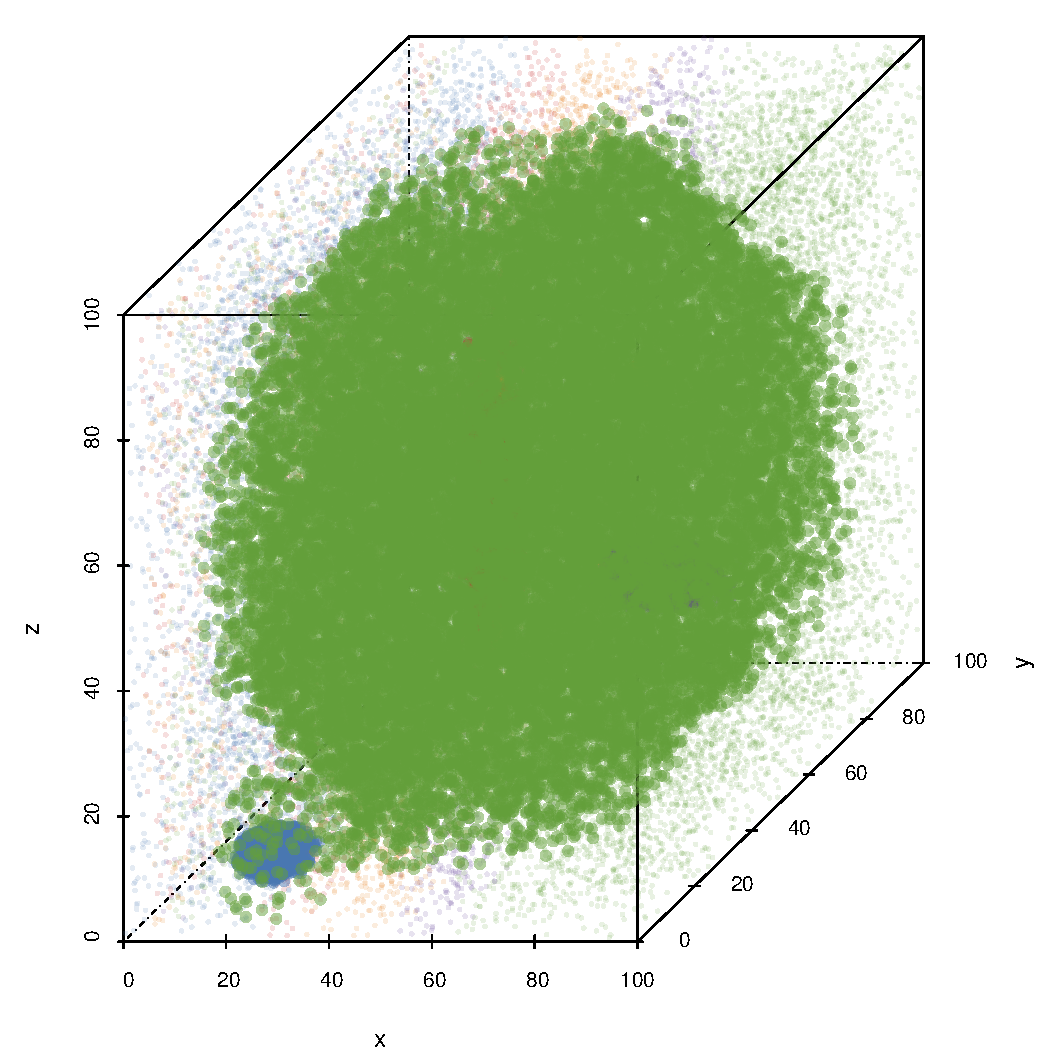
\includegraphics[keepaspectratio=true, width=\textwidth, height=0.23\textheight]{discussion/img/baakman_3_abs_error_mbeSmallerThansambe}
				\caption{Dataset \baakmanThree}
				\label{fig:discussion:performance:mbeLowerError:baakman3}
			\end{subfigure}			
			\caption{Low opacity scatter plot of dataset %
				\subref{fig:discussion:performance:mbeLowerError:ferdosi2} \ferdosiTwo, %
				\subref{fig:discussion:performance:mbeLowerError:baakman2} \baakmanTwo, %
				\subref{fig:discussion:performance:mbeLowerError:ferdosi3} \ferdosiThree, and %
				\subref{fig:discussion:performance:mbeLowerError:baakman3} \baakmanThree %
				with an overlay of high opacity larger points where the absolute error of \mbe is smaller than that of \sambe.}
			\label{fig:discussion:performance:multisphere:mbeLowerError}
		\end{figure}	
		The points where using fixed-shape kernels results in a smaller error in datasets \ferdosiTwo through \baakmanThree are emphasized in
		\cref{fig:discussion:performance:multisphere:mbeLowerError}. We contribute the boundary effect in these datasets to the same cause as the boundary effects in the datasets with a single Gaussian component. Interestingly the points in dataset \ferdosiThree and \baakmanThree where the absolute error of \mbe is lower approximate a sphere, contrary to the cube they define for dataset \ferdosiTwo and \baakmanTwo. It is our expectation that this is caused by smaller distance between the means of the Gaussian components and the boundary of the dataset. 
			% Define Ferdosi 3 Noise
			To test this we define dataset \ferdosiThreeNoise, this dataset replaces the uniform random background of \ferdosiThree with $\uniformDist{[-20, -20, -20]}{[120, 120, 120]}$. We adjust the number of points sampled from this component to ensure that its density is equal to that of the noise component of \ferdosiThree.
			% Is there any effect on the MSE
			Compared to \ferdosiThree, the overall \mse of both estimators has decreased slightly for \ferdosiThreeNoise, however the \mse of `Trivariate Gaussian 1' and 3 shows a small increase. 
			% Did the distance to the boundaries explain it?
			\Cref{fig:discussion:ferdosi3Noise:mbeLowerError} confirms that the spherical shape in \cref{fig:discussion:performance:mbeLowerError:ferdosi3,fig:discussion:performance:mbeLowerError:baakman3} is caused by the Gaussian near the boundary of the dataset. As the shape defined by the emphasized points is now a cubical instead of spherical. 
			% The Plots of Ferdosi 3 Noise
			\begin{figure}
				\centering
				\begin{subfigure}{0.23\textwidth}
					\centering
					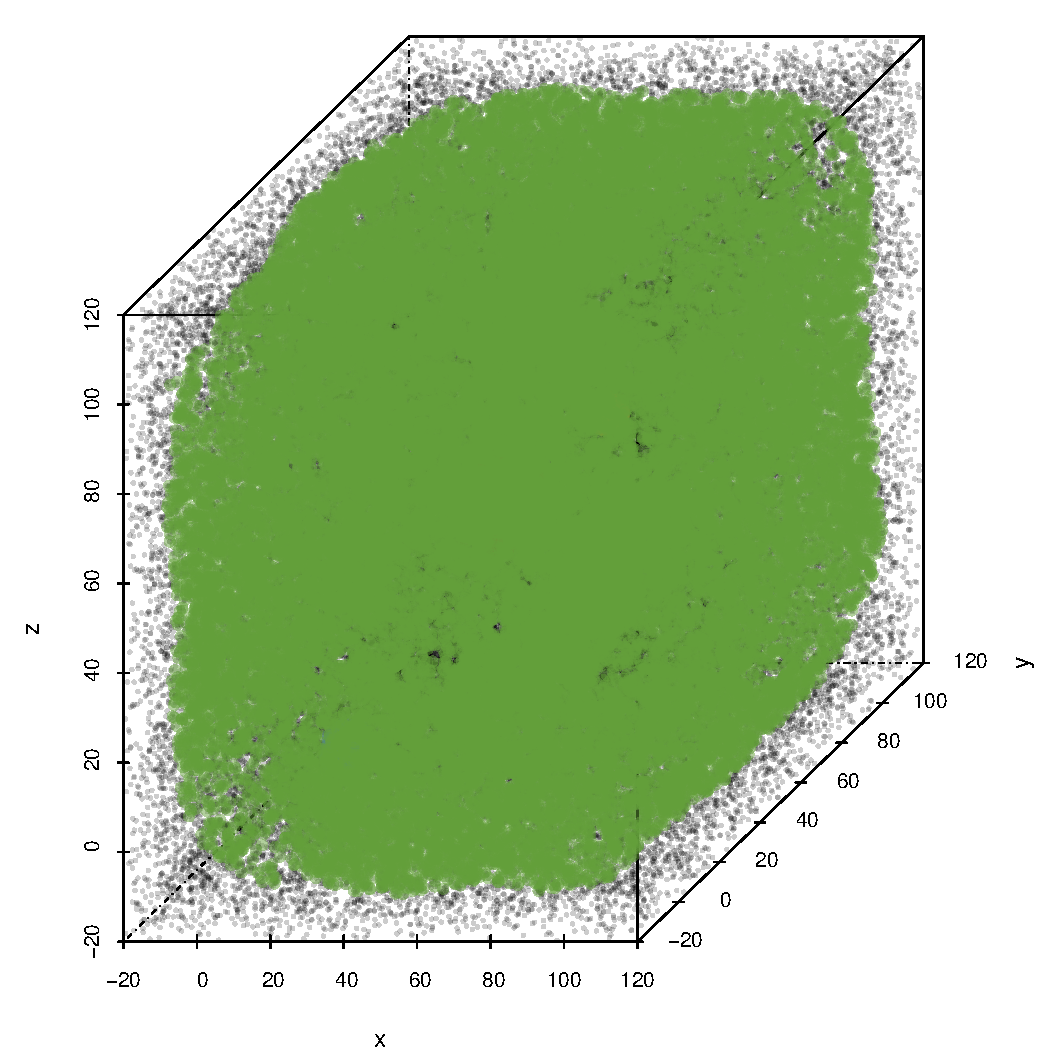
\includegraphics[keepaspectratio=true, width=\textwidth, height=0.23\textheight]{discussion/img/ferdosi_3_more_noise_abs_error_mbeSmallerThansambe.png}
					\caption{Absolute Error}
					\label{fig:discussion:ferdosi3Noise:mbeLowerError}
				\end{subfigure}		
				\begin{subfigure}{0.23\textwidth}
					\centering
					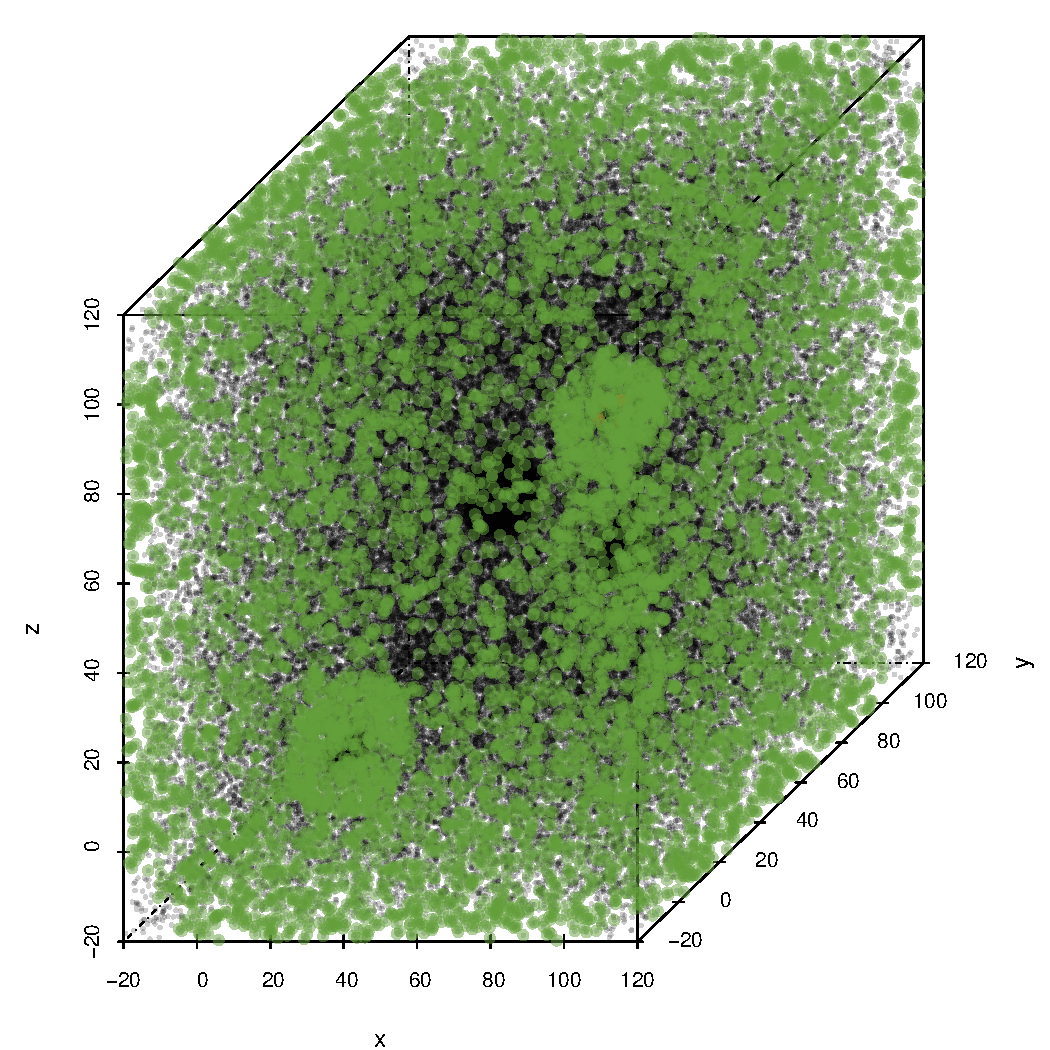
\includegraphics[keepaspectratio=true, width=\textwidth, height=0.23\textheight]{discussion/img/ferdosi_3_more_noise_anisotropy.png}
					\caption{Anisotropy}
					\label{fig:discussion:ferdosi3Noise:anisotropy}
				\end{subfigure}			
				\caption{Low opacity scatter plot of dataset \ferdosiThreeNoise with %
					\subref{fig:discussion:ferdosi3Noise:mbeLowerError} points where the absolute error of \mbe is lower than that of \sambe and %
					\subref{fig:discussion:ferdosi3Noise:anisotropy} points sampled from the Gaussian components with kernels whose anisotropy falls in the \nth{95} percentile of the complete dataset emphasized.}
				\label{fig:discussion:ferdosi3Noise}
			\end{figure}		

% Some conclusion
To conclude we have found that shape-adaptive kernels definitely improve performance in some cases, \eg near the boundary of the datasets and near the mean of some Gaussian components. Unfortunately in other cases the anisotropic kernels are detrimental, the difference in \mse between the two estimators show that on these datasets using symmetric kernels is slightly advantageous. 